\documentclass[simplex.tex]{subfiles}
% NO NEED TO INPUT PREAMBLES HERE
% packages are inherited; you can compile this on its own

\onlyinsubfile{
\title{NeuroData SIMPLEX Report: Subfile}
}

\begin{document}
\onlyinsubfile{
\maketitle
\thispagestyle{empty}

The following report documents the progress made by the labs of Randal~Burns and Joshua~T.~Vogelstein at Johns Hopkins University towards goals set by the DARPA SIMPLEX grant.

%%%% Table of Contents
\tableofcontents

%%%% Publications
\bibliographystyle{IEEEtran}
\begin{spacing}{0.5}
\section*{Publications, Presentations, and Talks}
\vspace{-20pt}
\nocite{*}
{\footnotesize	\bibliography{simplex}}
\end{spacing}
%%%% End Publications
}

\subsection{Science in the Cloud (SIC)}

A framework for \itshape{science in the cloud} (SIC) was developed which was
designed for extensibility of scientific findings. This work was
developed alongside a live demonstration, available at
\href{http://scienceinthe.cloud}{http://scienceinthe.cloud}, which illustrates this framework. There are
six key components which much be considered in sic: data storage, data
organization, interactive demos, virtualization, computing, and
deployment. The selection made for each of these components will have a
significant impact on available selections for the others. The final
product will be a highly interdependent network of tools and data.

\begin{figure}[h!]
\begin{cframed}
\centering
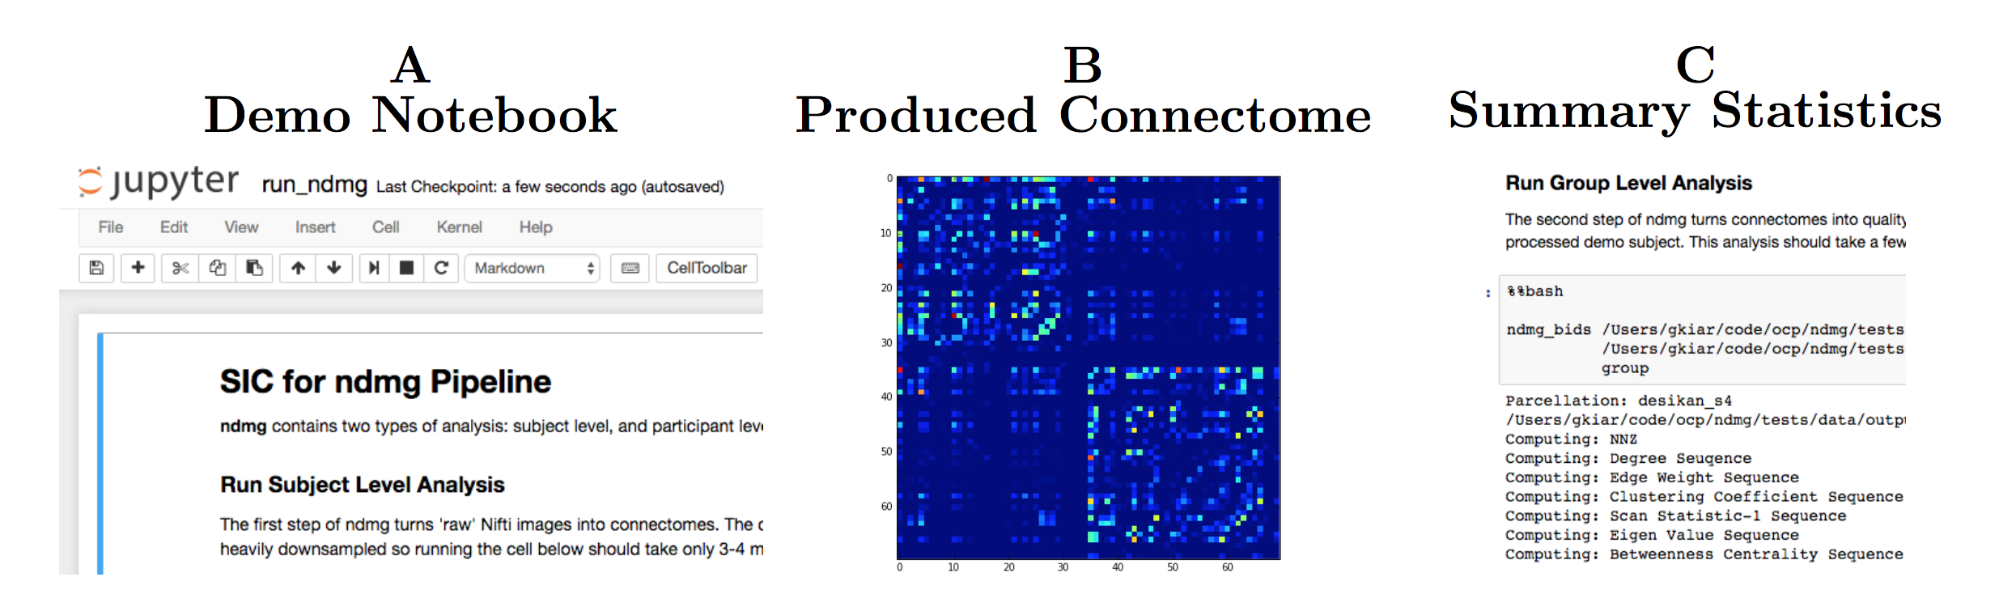
\includegraphics[width=0.95\textwidth]{./figs/sic.png}
\caption{
  States of the demo notebook in the cloud. A) A Jupyter notebook
  displaying descriptions and code snippets to be run for both
  connectome estimation and summary statistic computation. B) After
  running connectome generation an adjacency matrix will appear to
  provide a visualization. C) Summary statistic computation calculates
  several graph features and plots them in a multipanel figure. 
}
\label{fig:sic}
\end{cframed}
\end{figure}

We have refined our framework for science in the cloud (sic) and
submitted the manuscript to GigaScience. In particular, we have clearly
defined six crucial components to adopt this model of extensible
scientific tool production. These six components are: cloud data
storage, data organization, interactive demonstrations, virtualization,
deployment, and computing. Table~\ref{fig:sicTab} summarizes some tools for
each of these components, as well as the selection made in our
particular implementation of sic.


\begin{figure}[h!]
\begin{cframed}
\centering
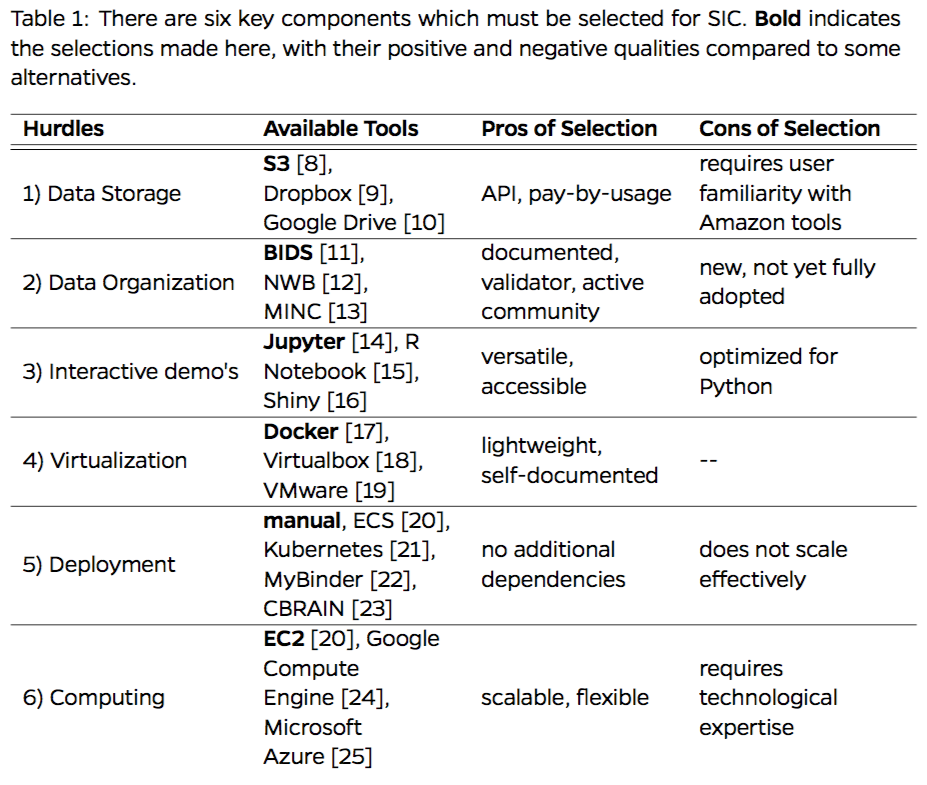
\includegraphics[width=0.85\textwidth]{./figs/sicTab.png}
\caption{
  Excerpted table from \cite{kiar2016}.
}
\label{fig:sicTab}
\end{cframed}
\end{figure}
\end{document}
